\documentclass{../../oss-apphys-exam}

\begin{document}
\genheader

\gentitle{C}{ROTATIONAL MOTION}

\genmultidirections

\gengravity

\raggedcolumns
\begin{multicols*}{2}
  \begin{questions}
    \question A meter stick of mass \SI{.1}{\kilo\gram} rests on a table as
    shown. A length of \SI{40}{\centi\metre} extends over the edge of the table.
    How far from the edge of the table could a \SI{.05}{\kilo\gram} mass be
    placed on the meter stick so that the stick just begins to tip?
    \begin{center}
      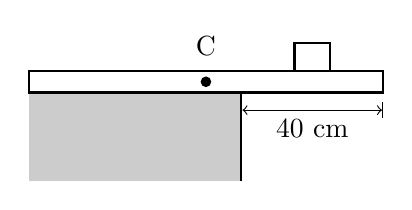
\begin{tikzpicture}[scale=4.5]
        \fill[gray!40](0,-.25) rectangle(.6,0);
        \begin{scope}[thick]
          \draw(0,0) rectangle(1,.06);
          \draw(.6,0)--(.6,-.25);
          \draw(.75,.06) rectangle (.85,.14);
        \end{scope}
        \draw[|<->|](.6,-.05)--(1,-.05) node[midway,below]{40 cm};
        \fill(.5,.03) circle(.015);
        \node at (.5,.13){C};
      \end{tikzpicture}
    \end{center}
    \begin{choices}
      \choice\SI{5}{\centi\metre}
      \choice\SI{10}{\centi\metre}
      \choice\SI{15}{\centi\metre}
      \choice\SI{20}{\centi\metre}
      \choice\SI{30}{\centi\metre}
    \end{choices}
    
    \question A metal bar of constant density and weight $W$ is attached to a
    pivot on the wall at point $P$ and supported by a rope that makes an angle
    of \ang{60} with the vertical wall. The reaction force exerted by the pivot
    on the bar at point P is best represented by which arrow?
    \cpic{.25}{metal-bar}
    \begin{choices}
      \choice{\Large $\nearrow$}
      \choice{\Large $\uparrow$}
      \choice{\Large $\downarrow$}
      \choice{\Large $\nwarrow$}
      \choice{\Large $\searrow$}
    \end{choices}
    \columnbreak
    
    \question A ballet dancer is spinning around a vertical axis with her arms
    fully extended. How are her angular momentum and kinetic energy affected
    as she pulls her arms in toward her body as she spins?
    \begin{choices}
      \choice Her angular momentum remains constant, but her kinetic energy
      increases.
      \choice Her angular momentum increases, but her kinetic energy remains
      constant.
      \choice Her angular momentum decreases, but her kinetic energy remains
      constant.
      \choice Her angular momentum increases, but her kinetic energy decreases.
      \choice Both her angular momentum and kinetic energy remain constant.
    \end{choices}
    
    \question A particle of mass $m$ moves with a constant speed $\varv$ at a
    distance $x_0$ parallel to the $y$-axis as shown. When the particle is in
    the position shown below, the magnitude of its angular momentum relative to
    the origin is
    \begin{center}
      \begin{tikzpicture}
        \fill(2,1.5) circle(.08);
        \begin{scope}[thick]
          \draw[->](-.2,0)--(3,0) node[right]{$x$} node[pos=0,below]{$O$};
          \draw[->](0,-.2)--(0,2.5) node[above]{$y$};
          \draw[dashed](0,1.5)--(2,1.5) node[pos=0,left]{$y_0$}
          --(2,0)node[below]{$x_0$};
        \end{scope}
        \draw[very thick,->](2,1.5)--(2,.5) node[midway,right]{$\varv$};
      \end{tikzpicture}
    \end{center}
    \begin{choices}
      \choice $m\varv x_0$
      \choice $m\varv y_0$
      \choice $m\varv\sqrt{x_0^2+y_0^2}$
      \choice $\dfrac{m\varv}{\sqrt{x_0^2+y_0^2}}$
      \choice zero
    \end{choices}
    \columnbreak
    
    \question A uniform rod of length $L$ and mass $m$ has a rotational inertia
    of $\dfrac1{12}mL^2$ about its center. A particle, also of mass $m$, is
    attached to one end of the stick. The combined rotational inertia of the
    stick and particle about the center of the rod is
    \begin{center}
      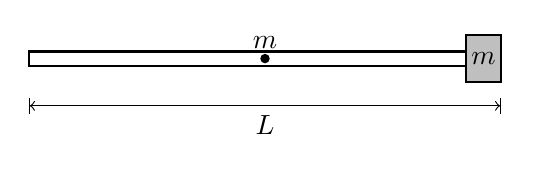
\begin{tikzpicture}[scale=3]
        \draw[thick](-1,-.03) rectangle (1,.03);
        \fill(0,0) circle(.02) node[above]{$m$};
        \draw[thick,fill=gray!50](.85,-.1) rectangle(1,.1) node[midway]{$m$};
        \draw[|<->|](-1,-.2)--(1,-.2) node[midway,below]{$L$};
      \end{tikzpicture}
    \end{center}
    \begin{choices}
      \choice$\dfrac{mL^2}3$
      \choice$\dfrac{12mL^2}{13}$
      \choice$\dfrac{13mL^2}{12}$
      \choice$\dfrac{mL^2}{156}$
      \choice$\dfrac{13mL^2}{156}$
    \end{choices}

    \question A hoop of radius $R$ and mass $m$ has a rotational inertia of
    $mR^2$. The hoop rolls without slipping along a horizontal floor with a
    constant speed $\varv$ and then rolls up a long incline. The hoop can roll
    up the incline to a maximum vertical height of
    \begin{center}
      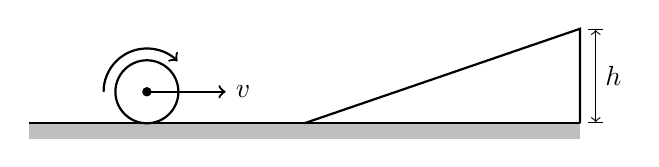
\begin{tikzpicture}
        \fill[gray!50](0,-.2) rectangle(7,0);
        \begin{scope}[thick]
          \draw(0,0)--(7,0);
          \draw(3.5,0)--(7,1.2)--(7,0);
          \draw(1.5,.4) circle(.4);
          \fill(1.5,.4) circle(.06);
          \draw[->](1.5,.4)--(2.5,.4) node[right]{$v$};
          \draw[->](.95,.4) arc(180:45:.55);
        \end{scope}
        \draw[|<->|](7.2,0)--(7.2,1.2) node[midway,right]{$h$};
      \end{tikzpicture}
    \end{center}
    \begin{choices}
      \choice$\dfrac{\varv^2}g$
      \choice$\dfrac{2\varv^2}{g}$
      \choice$\dfrac{\varv^2}{2g}$
      \choice$\dfrac{4\varv^2}{g}$
      \choice$\dfrac{\varv^2}{4g}$
    \end{choices}
    \columnbreak
    
    \question Two disks are fixed to a vertical axle that is rotating with a
    constant angular speed $\omega$. The smaller disk has a mass $m$ and a
    radius $r$, and the larger disk has a mass $2m$ and radius $2r$. The
    general equation for the rotational inertia of a disk of mass $M$ and
    radius $R$ is $\frac12MR^2$. The ratio of the angular momentum of the
    larger disk to the smaller disk is
    \cpic{.25}{2disks}
    \begin{choices}
      \choice $1:4$
      \choice $4:1$
      \choice $1:2$
      \choice $2:1$
      \choice $8:1$
    \end{choices}
    
    \question A light rod has a mass attached at each end. At one end is a
    \SI{6}{\kilo\gram} mass, and at the other end is a \SI{3}{\kilo\gram} mass.
    An axis can be placed at any of the points shown. Through which point
    should an axis be placed so that the rotational inertia is the greatest
    about that axis?
    \begin{center}
      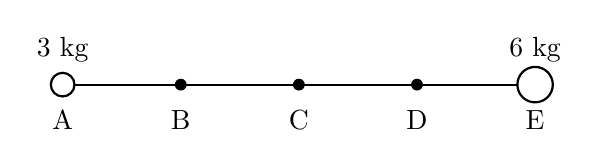
\begin{tikzpicture}[scale=1.5]
        \begin{scope}[thick]
          \draw(0,0) circle(.1);
          \draw(4,0) circle(.15);
          \draw(.1,0)--(3.85,0);
        \end{scope}
        \fill (1,0) circle(.05);
        \fill (2,0) circle(.05);
        \fill (3,0) circle(.05);
        \node at (0,-.3){A};
        \node at (1,-.3){B};
        \node at (2,-.3){C};
        \node at (3,-.3){D};
        \node at (4,-.3){E};
        \node at (0,.3){3 kg};
        \node at (4,.3){6 kg};
      \end{tikzpicture}
    \end{center}
    \begin{choices}
      \choice A
      \choice B
      \choice C
      \choice D
      \choice E
    \end{choices}
    \columnbreak
    
    \uplevel{
      \textbf{Question \ref{lightrod1}--\ref{lightrod2}}
      
      A light rod of negligible mass is pivoted at point $P$ a distance
      $L$ from one end as shown. A mass $m$ is attached to the left end of the
      rod at a distance of $3L$ from the pivot, and another mass $4m$ is
      attached to the other end a distance $L$ from the pivot. The system
      begins from rest in the horizontal position.
      \begin{center}
        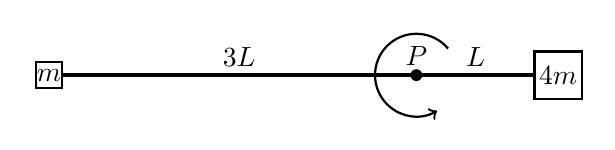
\begin{tikzpicture}[scale=1.5]
          \draw[very thick](-3,0)--(1,0);
          \draw[thick](1,-.2) rectangle(1.4,.2) node[midway]{$4m$};
          \draw[thick](-3,-.11) rectangle(-3.22,.11) node[midway]{$m$};
          \fill(0,0) circle(.05) node[above]{$P$};
          \node at (.5,.15){$L$};
          \node at (-1.5,.15){$3L$};
          \draw[thick,->,rotate=40](.35,0) arc(0:260:.35);
        \end{tikzpicture}
      \end{center}
    }
    
    \question The net torque acting on the system due to gravitational forces is
    \label{lightrod1}
    \begin{choices}
      \choice $4mgL$ clockwise
      \choice $3mgL$ clockwise
      \choice $3mgL$ counterclockwise
      \choice $mgL$ counterclockwise
      \choice $mgL$ clockwise
    \end{choices}
    
    \question The angular acceleration of the system when it is released from
    rest is
    \label{lightrod2}
    \begin{choices}
      \choice zero
      \choice $\dfrac{g}{5L}$
      \choice $\dfrac{g}{4L}$
      \choice $\dfrac{g}{13L}$
      \choice $\dfrac{g}L$
    \end{choices}

    \question Two wheels are attached to each other and fixed so that they can
    only turn together. The smaller wheel has a radius of $r$ and the larger
    wheel has a radius of $3r$. The two wheels can rotate together on a
    frictionless axle. Three forces act tangentially on the edge of the wheels
    as shown. The magnitude of the net torque acting on the system of wheels is
    \begin{center}
      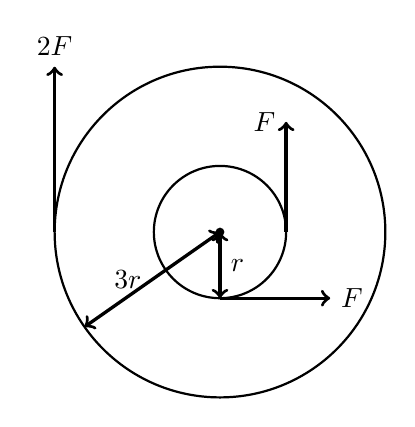
\begin{tikzpicture}[scale=.7]
        \begin{scope}[thick]
          \draw(0,0) circle(1.2);
          \draw(0,0) circle(3);
          \fill(0,0) circle(.08);
        \end{scope}
        \begin{scope}[very thick]
          \draw[<->](0,0)--(0,-1.2) node[midway,right]{$r$};
          \draw[<->,rotate=-55](0,0)--(0,-3) node[midway,left]{$3r$};
          \draw[->](0,-1.2)--(2,-1.2) node[right]{$\mb{F}$};
          \draw[->](1.2,0)--(1.2,2) node[left]{$\mb{F}$};
          \draw[->](-3,0)--(-3,3) node[above]{$2\mb{F}$};
        \end{scope}
      \end{tikzpicture}
    \end{center}
    \begin{choices}
      \choice $Fr$
      \choice $2Fr$
      \choice $3Fr$
      \choice $4Fr$
      \choice $6Fr$
    \end{choices}
    \columnbreak

    \question A disk is mounted on a fixed axle. The rotational inertia of the
    disk is $I$. The angular velocity of the disk is decreased from $\omega_i$
    to $\omega_f$ during a time $\Delta t$ due to friction in the axle. The
    magnitude of the average net torque acting on the wheel is
    \begin{choices}
      \choice $\dfrac{\omega_f-\omega_i}{\Delta t}$
      \choice $\dfrac{(\omega_f-\omega_i)^2}{\Delta t}$
      \choice $\dfrac{I(\omega_f-\omega_i)}{\Delta t}$
      \choice $\dfrac{I(\omega_f-\omega_i)^2}{\Delta t}$
      \choice $\dfrac{I(\omega_f-\omega_i)}{\Delta t^2}$
    \end{choices}
    
  \question The average power developed by the friction in the axle of the disk
    from the previous question to bring it to a complete stop is
    \begin{choices}
      \choice $\dfrac{\omega_i}{\Delta t}$
      \choice $\dfrac{\omega_i^2}{\Delta t}$
      \choice $\dfrac{I\omega_i}{2\Delta t}$
      \choice $\dfrac{I\omega_i^2}{\Delta t}$
      \choice $\dfrac{I\omega_i}{\Delta t^2}$
    \end{choices}    

    \question Astronauts are conducting an experiment in a negligible gravity
    environment. Two spheres of mass $m$ are attached to either end of a light
    rod. As the rod and spheres float motionless in space, an astronaut
    launches a piece of sticky clay, also of mass $m$, toward one of the spheres
    so that the clay strikes and sticks to the sphere perpendicular to the rod.
    Which of the following statements is true of the motion of the rod, clay,
    and spheres after the collision?
    \begin{center}
      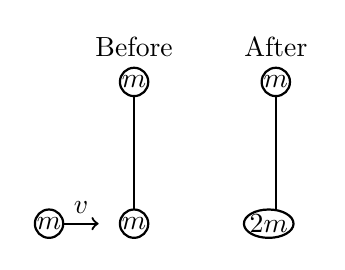
\begin{tikzpicture}[scale=.9]
        \begin{scope}[thick]
          \draw(0,0) circle(.2) node{$m$};
          \draw(0,2) circle(.2) node{$m$};
          \draw(0,.2)--(0,1.8);
          \draw(-1.2,0) circle(.2) node{$m$};
          \draw[->](-1,0)--(-.5,0) node[above left]{$v$};

          \draw(1.9,0) ellipse(.35 and .2) node{$2m$};
          \draw(2,2) circle(.2) node{$m$};
          \draw(2,.2)--(2,1.8);
        \end{scope}
        \node at (0,2.5) {Before};
        \node at (2,2.5) {After};
      \end{tikzpicture}
    \end{center}
    \begin{choices}
      \choice Linear momentum is not conserved, but angular momentum is
      conserved.
      \choice Angular momentum is not conserved, but linear momentum is
      conserved.
      \choice Kinetic energy is conserved, but angular momentum is not
      conserved.
      \choice Kinetic energy is conserved, but linear momentum is not conserved.
      \choice Both linear momentum and angular momentum are conserved, but
      kinetic energy is not conserved.
    \end{choices}
    
    \question A rod of mass $M$, length $L$, and rotational inertia $I$ hangs
    at rest from a frictionless axle as shown. A ball of mass $m$ with a speed
    $\varv$ strikes therod perpendicularly at the end of the rod. As a result
    of the collision, the ball stops. The angular speed of the rod immediately
    after the collision is
    \begin{center}
      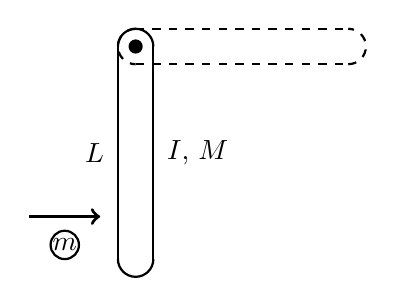
\begin{tikzpicture}[scale=.9]
        \fill(0,0) circle(.1);
        \begin{scope}[thick]
          \draw(.25,0) arc(0:180:.25);
          \draw(-.25,0)--(-.25,-3);
          \draw( .25,0)--( .25,-3);
          \draw(-.25,-3) arc(180:360:.25);
          \begin{scope}[dashed,rotate=90]
            \draw(.25,0) arc(0:180:.25);
            \draw(-.25,0)--(-.25,-3);
            \draw( .25,0)--( .25,-3);
            \draw(-.25,-3) arc(180:360:.25);
          \end{scope}
          \draw(-1,-2.8) circle(.2) node{$m$};
          \draw[very thick,->](-1.5,-2.4)--(-.5,-2.4)
          node[midway,above]{$\varv$};
          \node[left] at (-.3,-1.5) {$L$};
          \node[right] at (.3,-1.5) {$I$, $M$};
        \end{scope}
      \end{tikzpicture}
    \end{center}
    \begin{choices}
      \choice $\varv L$
      \choice $\dfrac{\varv}L$
      \choice $\dfrac{m\varv}I$
      \choice $\dfrac{m\varv L}I$
      \choice $\dfrac{m\varv}{IL}$
    \end{choices}
    \columnbreak

    \uplevel{
      \textbf{Questions \ref{hollow1}--\ref{hollow2}}

      A hollow sphere of mass $m$ and radius $R$ begins from rest at a height
      $h$ and rolls down a rough inclined plane. The rotational inertia of the
      hollow sphere is $\dfrac23mR^2$.
      \begin{center}
        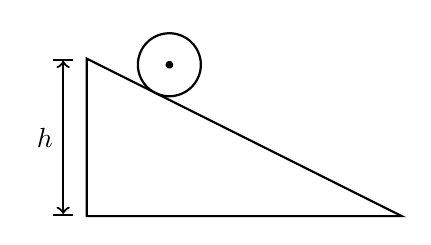
\begin{tikzpicture}
          \begin{scope}[thick]
            \draw(0,0)--(-4,0)--(-4,2)--cycle;
            \draw[|<->|](-4.3,2)--(-4.3,0) node[midway,left]{$h$};
          \end{scope}
          \begin{scope}[thick,rotate=-atan(2/4)]
            \draw(-3.5,.4) circle(.4);
            \fill(-3.5,.4) circle(.05);
          \end{scope}
        \end{tikzpicture}
      \end{center}
    }

    \question Which of the following diagrams best represents the forces acting
    on  the sphere as it rolls down the plane?
    \begin{choices}
    \choice 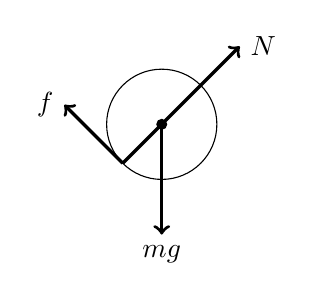
\begin{tikzpicture}[scale=.7]
      \draw(0,0) circle(1);
      \fill(0,0) circle(.1);
      \begin{scope}[very thick,->]
        \draw (0,0)--(0,-2) node[below]{$mg$};
        \draw[rotate=45](-1,0)--(2,0) node[right]{$N$};
        \draw[rotate=45](-1,0)--(-1,1.5) node[left]{$f$};
      \end{scope}
    \end{tikzpicture}

    \choice 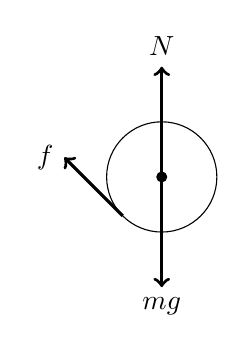
\begin{tikzpicture}[scale=.7]
      \draw(0,0) circle(1);
      \fill(0,0) circle(.1);
      \begin{scope}[very thick,->]
        \draw (0,0)--(0,-2) node[below]{$mg$};
        \draw (0,0)--(0,2) node[above]{$N$};
        \draw[rotate=45](-1,0)--(-1,1.5) node[left]{$f$};
      \end{scope}
    \end{tikzpicture}

    \choice 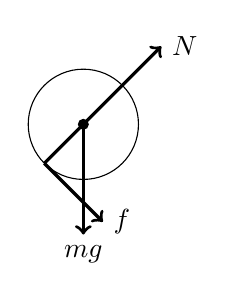
\begin{tikzpicture}[scale=.7]
      \draw(0,0) circle(1);
      \fill(0,0) circle(.1);
      \begin{scope}[very thick,->]
        \draw (0,0)--(0,-2) node[below]{$mg$};
        \draw[rotate=45](-1,0)--(2,0) node[right]{$N$};
        \draw[rotate=45](-1,0)--(-1,-1.5) node[right]{$f$};
      \end{scope}
    \end{tikzpicture}

    \choice 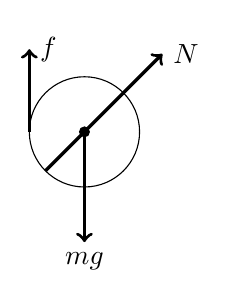
\begin{tikzpicture}[scale=.7]
      \draw(0,0) circle(1);
      \fill(0,0) circle(.1);
      \begin{scope}[very thick,->]
        \draw (0,0)--(0,-2) node[below]{$mg$};
        \draw[rotate=45](-1,0)--(2,0) node[right]{$N$};
        \draw(-1,0)--(-1,1.5) node[right]{$f$};
      \end{scope}
    \end{tikzpicture}
      
    \choice 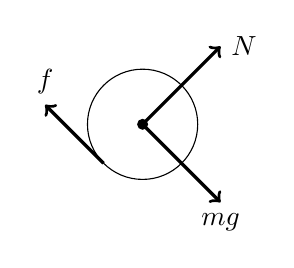
\begin{tikzpicture}[scale=.7]
      \draw(0,0) circle(1);
      \fill(0,0) circle(.1);
      \begin{scope}[very thick,->]
        \draw[rotate=45](0,0)--(0,-2) node[below]{$mg$};
        \draw[rotate=45](0,0)--(2,0) node[right]{$N$};
        \draw[rotate=45](-1,0)--(-1,1.5) node[above]{$f$};
      \end{scope}
    \end{tikzpicture}
    \end{choices}
    \label{hollow1}
    \columnbreak
    
    \question The speed of the sphere when it reaches the bottom of the plane is
    \begin{choices}
      \choice $\dfrac{8gh}5$
      \choice $\dfrac{6gh}5$
      \choice $\dfrac{5gh}6$
      \choice $\dfrac{7gh}{10}$
      \choice $\dfrac{gh}2$
    \end{choices}
    \label{hollow2}
    \columnbreak
    
    \question One end of a stick of length $L$, rotational inertia $I$, and
    mass $m$ is pivoted on an axle with negligible friction at point $P$. The
    other end is tied to a string and held in a horizontal position. When the
    string is cut, the stick rotates counterclockwise. The angular speed
    $\omega$ of the stick when it reaches the bottom of its swing is
    \cpic{.32}{end-of-stick}
    \begin{choices}
      \choice $\dfrac{mgL}I$
      \choice $\sqrt{\dfrac{mgL}I}$
      \choice $\sqrt{\dfrac{2mgL}I}$
      \choice $\sqrt{\dfrac{mgL}{2I}}$
      \choice $\sqrt{\dfrac{4mgL}I}$
    \end{choices}
  \end{questions}
\end{multicols*}
\newpage

\genfreetitle{C}{ROTATIONAL MOTION}{6}

\genfreedirections

% TAKEN FROM THE 2015 AP PHYSICS C FREE-RESPONSE QUESTION MECH 3
\begin{center}
  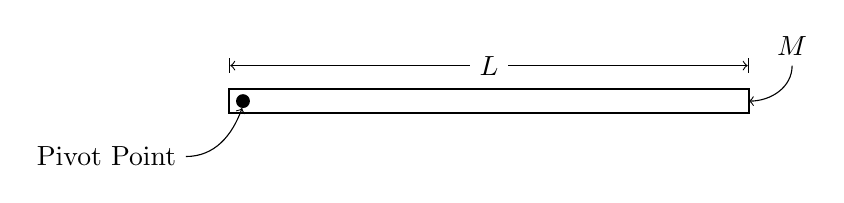
\begin{tikzpicture}[scale=1.1]
    \draw[thick](0,0) rectangle(6,.28);
    \fill(.16,.14) circle(.08);
    \draw[|<->|](0,.55)--(6,.55) node[midway,fill=white]{$L$};
    \draw[<-](6,.14) to[in=270,out=0](6.5,.55) node[above]{$M$};
    \draw[<-](.15,.06) to[in=0,out=250](-.5,-.5) node[left]{Pivot Point};
  \end{tikzpicture}
\end{center}
\begin{questions}
  \question A uniform, thin rod of length $L$ and mass $M$ is allowed to pivot
  about its end, as shown in the figure above.
  \begin{parts}
    \part Using integral calculus, derive the rotational inertia for the rod
    around its end to show that it is $ML^2/3$.
    
    \uplevel{
      \begin{center}
        \begin{tikzpicture}[scale=1.1]
          \draw[thick,dashed](0,.28) rectangle(.28,-5.72);
          \draw[thick,fill=white](0,0) rectangle(6,.28);
          \fill(.16,.14) circle(.08);
          \node[right] at (6,.14){$A$};
          \node[below] at (.14,-5.72){$B$};
          \draw[->,very thick](3,-.15) arc(-5:-85:2.8);
          \draw[thick,fill=white](.16,.14)--(.06,.7)--(.26,.7)--cycle;
          \fill[gray](-.4,.7) rectangle(.7,.9);
          \draw[thick](-.4,.7)--(.7,.7);
        \end{tikzpicture}
      \end{center}
      The rod is fixed at one end and allowed to fall from the horizontal
      position $A$ through the vertical position $B$.
    }
      
    \part Derive an expression for the velocity of the free end of the rod at
    position $B$. Express your answer in terms of $M$, $L$, and physical
    constants, as appropriate.
  
    \uplevel{
      An experiment is designed to test the validity of the expression found
      in part (b). A student uses rods of various lengths that all have a
      uniform mass distribution. The student releases each of the rods from
      the horizontal position $A$ and uses photogates to measure the velocity
      of the free end at position $B$. The data are recorded below.
      \begin{center}
        \def\arraystretch{1.45}
        \begin{tabular}{|c|c|c|c|c|c|c|}
          \hline
          Length (m)     & 0.25 & 0.50 & 0.75 & 1.00 & 1.25 & 1.50\\\hline
          Velocity (m/s) & 2.7  & 3.8  & 4.6  & 5.2  & 5.8  & 6.3 \\\hline
          & & & & & & \\\hline
          & & & & & & \\\hline
        \end{tabular}
        \def\arraystretch{1}
      \end{center}
    }

    \part Indicate below which quantities should be graphed to yield a straight
    line whose slope could be used to calculate a numerical value for the
    acceleration due to gravity $g$.

    \vspace{.1in}Horizontal axis: \underline{\hspace{1in}}

    \vspace{.1in}Vertical axis: \underline{\hspace{1in}}

    \vspace{.1in}Use the remaining rows in the table above, as needed, to
    record any quantities that you indicated that are not given. Label each row
    you use and include units.

    \part Plot the straight line data points on the grid below. Clearly scale
    and label all axes, including units as appropriate. Draw a straight line
    that best represents the data.
    \begin{center}
      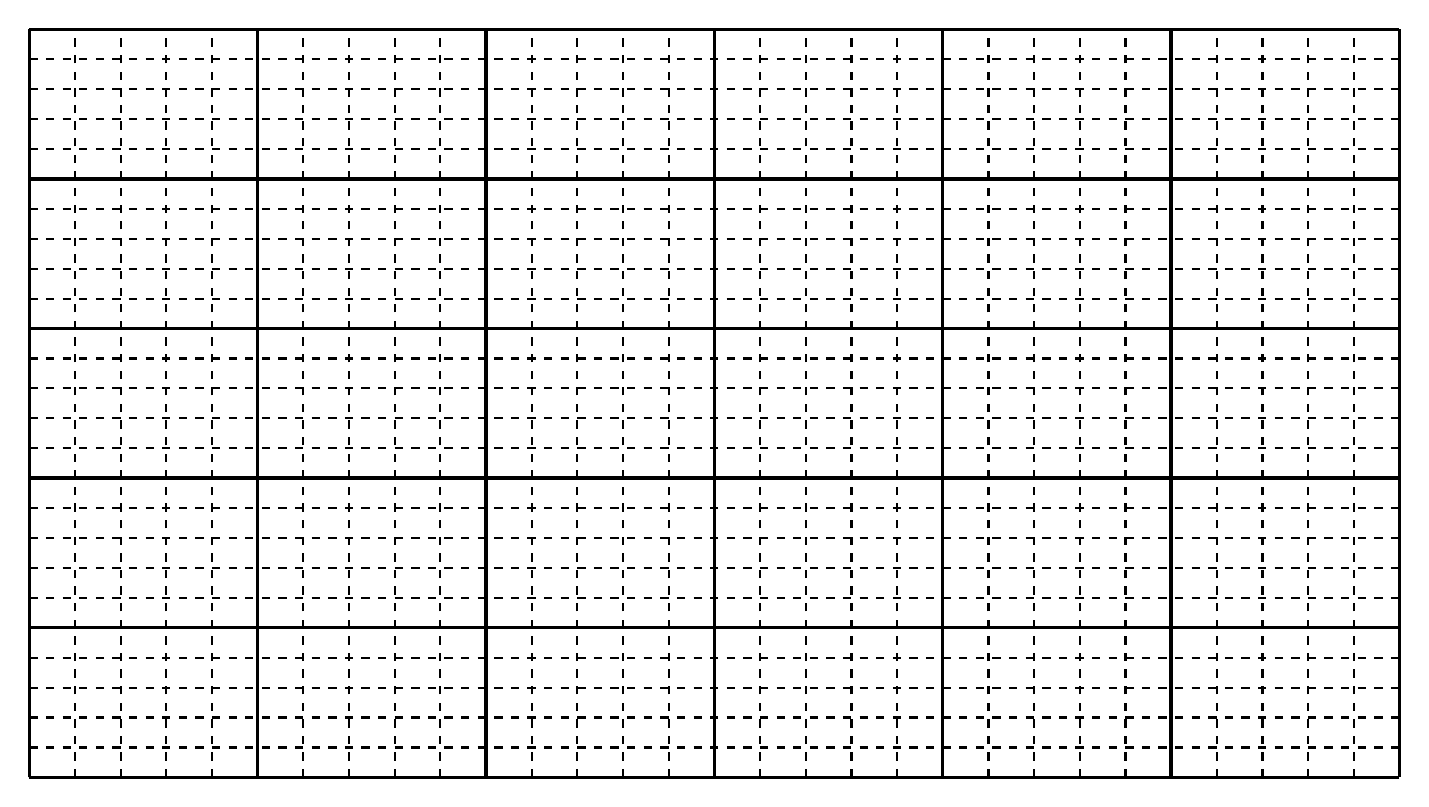
\begin{tikzpicture}[xscale=.58,yscale=.38]
        \draw[dashed,thick](0,0) grid(30,25);
        \draw[step=5,very thick](0,0) grid(30,25);
      \end{tikzpicture}
    \end{center}
    
    \part
    \begin{subparts}
      \subpart Using your straight line, determine an experimental value for
      $g$.
      \subpart Describe two ways in which the effects of air resistance could
      be reduced.
    \end{subparts}
  \end{parts}
  \newpage

  % THIS IS ACTUALLY A PRETTY GOOD QUESTION THAT I USE IN CLASS EXAMPLE
%  \question A uniform sphere of mass $M$ and radius $R$ is free to rotate,
%  without friction, about a horizontal axis through its center. A string is
%  wrapped around the sphere and is attached to a body of mass $m$ as shown in
%  the figure below. Find
%  \begin{center}
%    \begin{tikzpicture}[scale=.6]
%      \tikzstyle{balloon}=[ball color=red!80!gray!50];
%      \shade[balloon] (0,0) circle (2);% node[below right]{$m$};
%      \draw(0,0) circle(2);
%      \draw[fill=gray](0,0) circle(.2);
%      \draw[thick](2,0)--(2,-4);
%      \draw[fill=yellow!80!gray!50](1.5,-4) rectangle(2.5,-5)
%      node[midway,black]{$m$};
%      \draw[ultra thick,red!80!black,->](2,-4)--(2,-1.8)
%      node[pos=.9,right,black]{$T$};
%    \end{tikzpicture}
%  \end{center}
%  \begin{parts}
%    \part the acceleration of the body, and
%    \part the tension in the string.
%  \end{parts}
%  \newpage

  % TAKEN FROM THE 2004 AP PHYSICS C MECHANICS EXAM FREE-RESPONSE QUESTION 2
  \uplevel{
    \begin{center}
      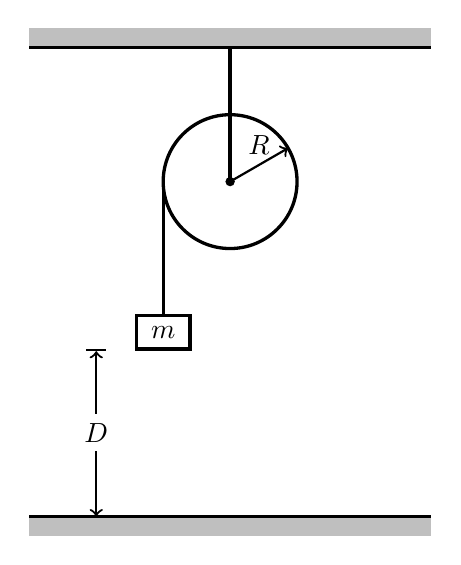
\begin{tikzpicture}[scale=.85]
        \draw[very thick](0,0) circle(1);
        \fill(0,0) circle(.07);
        \draw[very thick](0,0)--(0,2);
        \fill[gray!50](-3,2) rectangle(3,2.3);
        \draw[very thick](-3,2)--(3,2);
        \draw[thick,->,rotate=30](0,0)--(1,0) node[midway,above]{$R$};
        \draw[very thick](-1,0)--(-1,-2);
        \draw[very thick](-1.4,-2) rectangle(-.6,-2.5) node[midway]{$m$};
        \draw[thick,|<->](-2,-2.5)--(-2,-5) node[midway,fill=white]{$D$};
        \fill[gray!50](-3,-5) rectangle(3,-5.3);
        \draw[very thick](-3,-5)--(3,-5);
      \end{tikzpicture}
    \end{center}
  }
  \question A solid disk of unknown mass and known radius $R$ is used as a
  pulley in a lab experiment, as shown above. A small block of mass $m$ is
  attached to a string, the other end of which is attached to the pulley and
  wrapped around it several times. The block of mass $m$ is released from rest
  and takes a time $t$ to fall the distance $D$ to the floor.
  \begin{parts}
    \part Calculate the linear acceleration $a$ of the falling block in terms
    of the given quantities.

    \part The time $t$ is measured for various heights $D$ and the data are
    recorded in the following table.
    \begin{center}
      \begin{tabular}{|c|c|}
        \hline
        $D$ (m) & $t$ (s)\\\hline
        0.5 & 0.68\\\hline
        1   & 1.02\\\hline
        1.5 & 1.19\\\hline
        2   & 1.38\\\hline
      \end{tabular}
    \end{center}
    \begin{subparts}
      \subpart What quantities should be graphed in order to best determine the
      acceleration of the block? Explain your reasoning.

      \subpart On the grid below, plot the quantities determined in (b)i.,
      label the axes, and draw the best-fit line to the data.
      
      \vspace{.1in}
      \begin{center}
        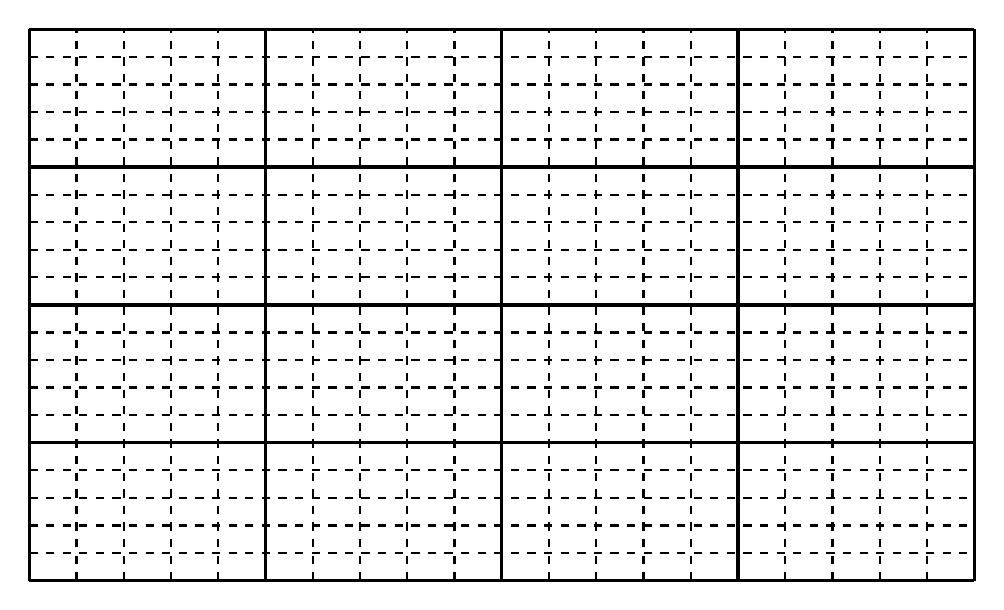
\begin{tikzpicture}[xscale=.6,yscale=.35]
          \draw[thick,dashed](0,0) grid(20,20);
          \draw[very thick,step=5](0,0) grid(20,20);
        \end{tikzpicture}
      \end{center}\vspace{.2in}
      
      \subpart Use your graph to calculate the magnitude of the acceleration.
    \end{subparts}

    \part Calculate the rotational inertia of the pulley in terms of $m$, $R$,
    $a$, and fundamental constants.

    \part The value of acceleration found in (b)iii, along with numerical
    values for the given quantities and your answer to (c), can be used to
    determine the rotational inertia of the pulley. The pulley is removed from
    its support and its rotational inertia is found to be greater than this
    value. Give one explanation for this discrepancy.
  \end{parts}
  \newpage
  
%  \question A uniform cylinder of mass $M$ and radius $R$ has a string wrapped
%  around it. The string is held fixed, and the cylinder falls vertically as
%  shown in the figure below. Find
%  \begin{center}
%    \begin{tikzpicture}[scale=.5]
%      \draw[fill=yellow!80!gray!50](0,0) circle(2);
%      \draw[thick](2,0)--(2,5);
%      \draw[ultra thick,red!80!black,->](2,0)--(2,3) node[pos=.9,right]{$T$};
%    \end{tikzpicture}
%  \end{center}
%  \begin{parts}
%    \part the acceleration of the body, and
%    \part the tension in the string.
%  \end{parts}
%  \newpage

  \uplevel{
    \cpic{.65}{disc1}
  }

  \question A large circular disk of mass $m$ and radius $R$ is initially
  stationary on a horizontal icy surface. A person of mass $m/2$ stands on the
  edge of the disk. Without slipping on the disk, the person throws a large
  stone of mass $m/20$ horizontally at initial speed $\varv_0$ from a height
  $h$ above the ice in a radial direction, as shown in the figures above. The
  coefficient of friction between the disk and the ice is $\mu$. All velocities
  are measured relative to the ground. The time it takes to throw the stone is
  negligible. Express all algebraic answers in terms of $m$, $R$, $\varv_0$,
  $h$, $m$, and fundamental constants, as appropriate.
  \begin{parts}
    \part Derive an expression for the length of time it will take the stone to
    strike the ice.
    
    \part Assuming that the disk is free to slide on the ice, derive an
    expression for the speed of the disk and person immediately after the stone
    is thrown.
    
    \part Derive an expression for the time it will take the disk to stop
    sliding.
  
    \uplevel{
      \begin{center}
        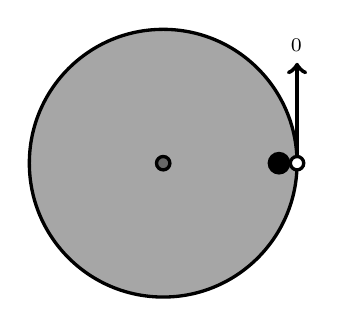
\begin{tikzpicture}[scale=.85]
          \draw[very thick,fill=gray!70](0,0) circle(2);
          \draw[very thick,fill=black!60](0,0) circle(.1);
          \draw[very thick,fill=white](2,0) circle(.1);
          \fill (1.73,0) circle(.17);
          \draw[ultra thick,->](2,.1)--(2,1.5) node[above]{$\varv_0$};
        \end{tikzpicture}

        Top View
      \end{center}
      The person now stands on a similar disk of mass $m$ and radius $R$ that
      has a fixed pole through its center so that it can only rotate on the
      ice. The person throws the same stone horizontally in a tangential
      direction at initial speed $\varv_0$, as shown in the figure above. The
      rotational inertia of  the disk is $mR^2/2$.
    }

    \part Derive an expression for the angular speed $\omega$ of the disk
    immediately after the stone is thrown.\label{partd}
    
    \part The person now stands on the disk at rest $R/2$ from the center of the
    disk. The person now throws the stone horizontally with a speed $\varv_0$ in
    the same direction as in part (\ref{partd}). Is the angular speed of the
    disk immediately after throwing the stone from this new position greater
    than, less than, or equal to the angular speed found in part (\ref{partd})?
    Justify your answer.
    
    \vspace{.1in}
    \underline{\hspace{.3in}} Greater than\hspace{.2in}
    \underline{\hspace{.3in}} Less than\hspace{.2in}
    \underline{\hspace{.3in}} Equal to
  \end{parts}
  \newpage
  
  \question A uniform ball of radius $r$ rolls without slipping along the
  loop-the-loop track in the figure below. The ball starts at rest at a height
  of $h$ above the bottom of the loop.
  \cpic{.55}{roll-ball}
  \begin{parts}
    \part If it is not to leave the track at the top of the loop, what is the
    least value $h$ can have (in terms of radius $R$ of the loop)?

    \part What would $h$ have to be if, instead of rolling, the ball slides
    without friction?
  \end{parts}
  \newpage
  
  \begin{center}
    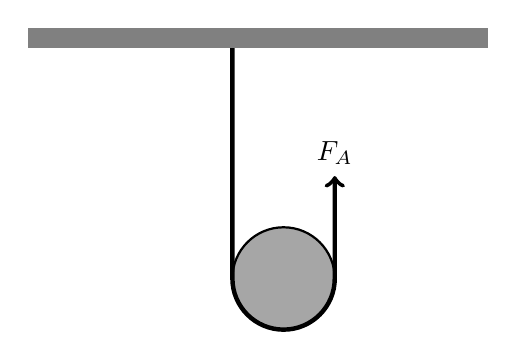
\begin{tikzpicture}[scale=.65]
      \fill[gray!70](0,0) circle(1);
      \draw[ultra thick,->](-1,4.5)--(-1,0) arc(180:360:1)
      --(1,2) node[above]{$F_A$};
      \draw[thick](-1,0) arc(180:0:1);
      \fill[gray](-5,4.5) rectangle(4,4.9);
    \end{tikzpicture}
  \end{center}
  \question A disk of mass $M =\SI{2.}{\kilo\gram}$ and radius
  $R=\SI{.10}\metre$ is supported by a rope of negligible mass, as shown
  above. The rope is attached to the ceiling at one end and passes under the
  disk. The other end of the rope is pulled upward with a force $F_A$. The
  rotational inertia of the disk around its center is $MR^2/2$.
  \begin{parts}
    \part Calculate the magnitude of the force $F_A$ necessary to hold the disk
    at rest.

    \uplevel{
      At time $t=0$, the force $F_A$ is increased to 12 N, causing the disk to
      accelerate upward. The rope does not slip on the disk as the disk rotates.
    }

    \part Calculate the linear acceleration of the disk.
    
    \part Calculate the angular speed of the disk at $t=\SI{3.}\second$.
    
    \part Calculate the increase in total mechanical energy of the disk from
    $t=0$ to $t=\SI{3.}\second$.
    
    \part The disk is replaced by a hoop of the same mass and radius. Indicate
    whether the linear acceleration of the hoop is greater than, less than, or
    the same as the linear acceleration of the disk. Justify your answer.

    \vspace{.1in}   
    \underline{\hspace{.3in}} Greater than\hspace{.2in}
    \underline{\hspace{.3in}} Less than\hspace{.2in}
    \underline{\hspace{.3in}} The same as
  \end{parts}
\end{questions}
\end{document}
